\section{Methods}

\subsection{Model}
\begin{itemize}

\item 
\richel{TODO: move to Introduction}
Current phylogenetic tools assume that only a single speciation event 
can occur at any given time.
While this assumption is useful to construct a wide variety of successful 
models (e.g \cite{Maddison2007biSSE}, \cite{Valente2015}, 
\cite{etienne2012diversity}, \cite{etienne2014estimating}),
they disallow for environmental changes that trigger speciations 
in multiple clades at a same point in time. 

\item 
\richel{TODO: move to Introduction}
In the MBD model, parameters $\lambda$ and $\mu$ correspond, respectively, 
to the common per-species speciation and extinction rates present 
also in the standard BD model. 
Additionally, MBD relies on two additional parameters. 
Parameter $\nu$ is the rate at which an environmental change is triggered.
When such event is triggered, 
all species present in the phylogeny at that moment
have a probability $q$ to speciate at that time, which is 
independent on $\lambda$. 
Polytomies are not allowed in such process 
as each species can speciate only once at the time.

\item 
\richel{TODO: move to Introduction}
It is also possible to write down a likelihood function 
for such processes as in \cite{mbd}.
    
\end{itemize}

\subsection{Simulations}
\begin{itemize}

\item To investigate the effect of $s$ on $e$, we simulate phylogenies
for different values of $s$ spread equally from zero (no multiple-birth
event, thus a BD model) to one (species are created only from multiple-birth
events) and three intermediate values of 0.25, 0.5 and 0.75. Aggregating all
components of $s$, we show the effect of $s$ on $e$ in figure \ref{fig:1}.

\item To see the effect of the number of taxa on the relation 
between $s$ and $e$, we simulate phylogenies
for different number of extant taxa $n$. We use values of $n$
of 50, 100 and 200 extant taxa, as this will result in phylogenies
that are big enough to be useful, yet small of enough to
be computationally feasible. For the different values of $n$, we show
the relation between $s$ and $e$ in figure \ref{fig:5} and its effect
on the variance of $e$ in figure \ref{fig:6}.

\item To see the effect of the extinction rate on the relation 
between $s$ and $e$, we simulate phylogenies
with different extinction rates $\mu$. We use values of $\mu$
of 0.0, 0.1 and 0.2. An extinction rate of zero has two features:
(1) the model falls back to a pure multiple-birth model, 
(2) all multiple-birth events are observed.
For the different values of $\mu$, we show
the relation between $s$ and $e$ in figure \ref{fig:2}.

\item We start simulating $N_{S} = 1000$ MBD trees,
with either 50, 100 and 200 taxa.

\item From each MBD tree, a DNA sequence alignment is simulated. 
For each sequence alignment we then perform a Bayesian analysis 
to recover a posterior distribution of trees, 
each composed of $N_{P}$ phylogenies. 
Such analysis is performed using 
the 'pirouette' package (\cite{pirouette}) to call the BEAST2 tool 
suite from R. 
We let the Bayesian analysis assume a BD prior in both cases, 
to investigate the extent of the error we make under this assumption.

\item For each tree generated under the MBD model 
we aim to generate a "twin" tree under the BD model. 
With the word "twin" 
we denote a tree generated starting from the respective MBD tree, 
in order to perform a fair comparison with it. 
This operation has to be done, 
because we want to compare two trees 
that are generated by different processes. 
To do so we infer the parameters $\lambda_{BD}$ and $\mu_{BD}$ 
from the MBD maximizing the likelihood under a BD model. 
To perform this operation we use the function "\texttt{bd\_ML}" 
from the package "\texttt{DDD}" (\cite{etienne2012diversity}). 

\item We then exploit such parameters to generate a BD tree 
using the function "\texttt{tess.sim.taxa.age}" 
from the package "\texttt{TESS}" (\cite{Hoehna2013}). 
We simulate the tree in such a way the new tree 
has the same number of tips and the same crown age as the MBD tree. 
We furthermore require that the BD tree conserve the topology of the MBD tree.
We have hypothesis H4 that, compared to the MBD trees, 
the error will be less in the BD twin tree.
The difference between the errors made in MBD and twin BD trees indicates
the impact the MBD process has on the error we make in inference using a
contemporary BD prior.

\begin{figure}[!htbp]
  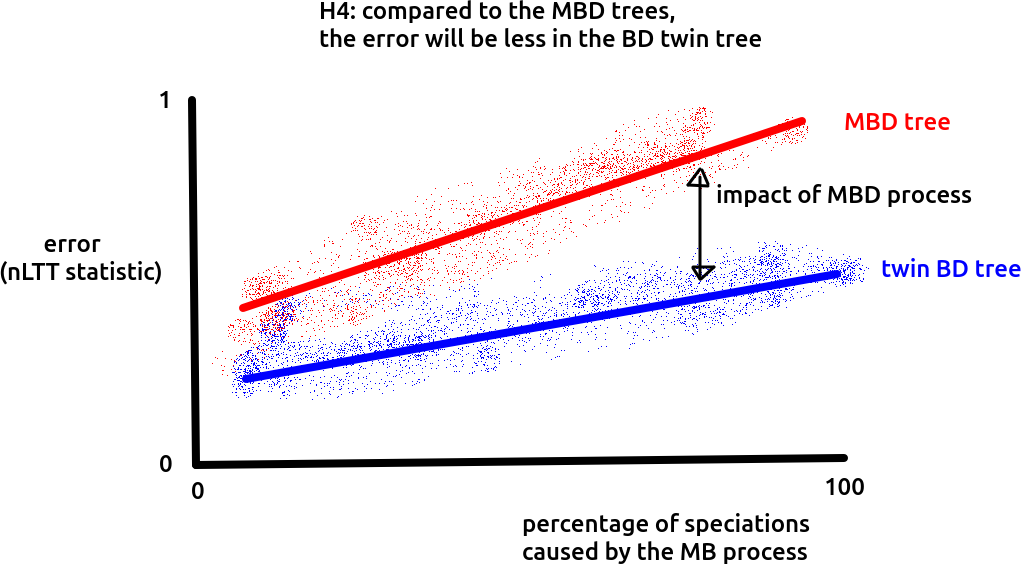
\includegraphics[width=\textwidth]{razzo-figures/fig_h_4.png}
  \caption{
    Hypothesis 4: compared to the MBD trees, 
    the error will be less in the BD twin tree
  }
  \label{fig:h_4}
\end{figure}

We want the MBD and twin BD trees to contain the same amount of information, 
i.e. the same number of DNA mutations and the same number of taxa at the present:

\begin{equation}
m_{MBD} = m_{BD} \label{m equivalence}
\end{equation} 

The expected number of mutations $m$ of a phylogeny 
with crown age $-T$ (with $T>0$) in fact is given by
\richel{
  So one of use likes '-T', the other likes 'T'. How to resolve this?
}

\begin{equation}
m = L \cdot \rho \cdot \int_{0}^{T} n(t)\ dt \label{m calculation}
\end{equation}

where $L$ is the number of DNA nucleotides, 
$\rho$ is the per-site per-species mutation rate and
$n(t)$ the number of species at each time.

The parameter we'll tune is $\rho$ ... \richel{elaborate here :-)}

Since we cannot know $n_{BD}(t)$ before running simulations
we need to replace it with a proxy. 
For this reason we will use the average number of
species in time according to the BD model. 
It's well known that this is equal to \gio{insert proper citation}

\begin{equation}
    <n_{BD}>(t) = n_{0} \cdot e^{(\mu_{BD} - \lambda_{BD})t} \label{BD average n}
\end{equation}

where $n_{0} = n_{BD}(-T) = n_{MBD}(-T)$ is the initial number of species 
at the crown age.
From \ref{m equivalence}, \ref{m calculation} and \ref{BD average n} follows:

\begin{equation}
    m_{MBD} = 
    L \cdot \rho \cdot \int_{0}^{T} <n_{BD}>(t)\ dt 
    \\ =
    L \cdot \rho \cdot n_{0} \cdot \left[ \frac{e^{(\mu_{BD} - \lambda_{BD})T} - 1}{\mu_{BD} - \lambda_{BD}} \right]
\end{equation}

If we set $\mu_{BD} = \mu_{MBD}$ and reverse this relation 
we can extrapolate the value of $\lambda_{BD}$ to use to generate BD trees.

\begin{figure}[!htbp]
  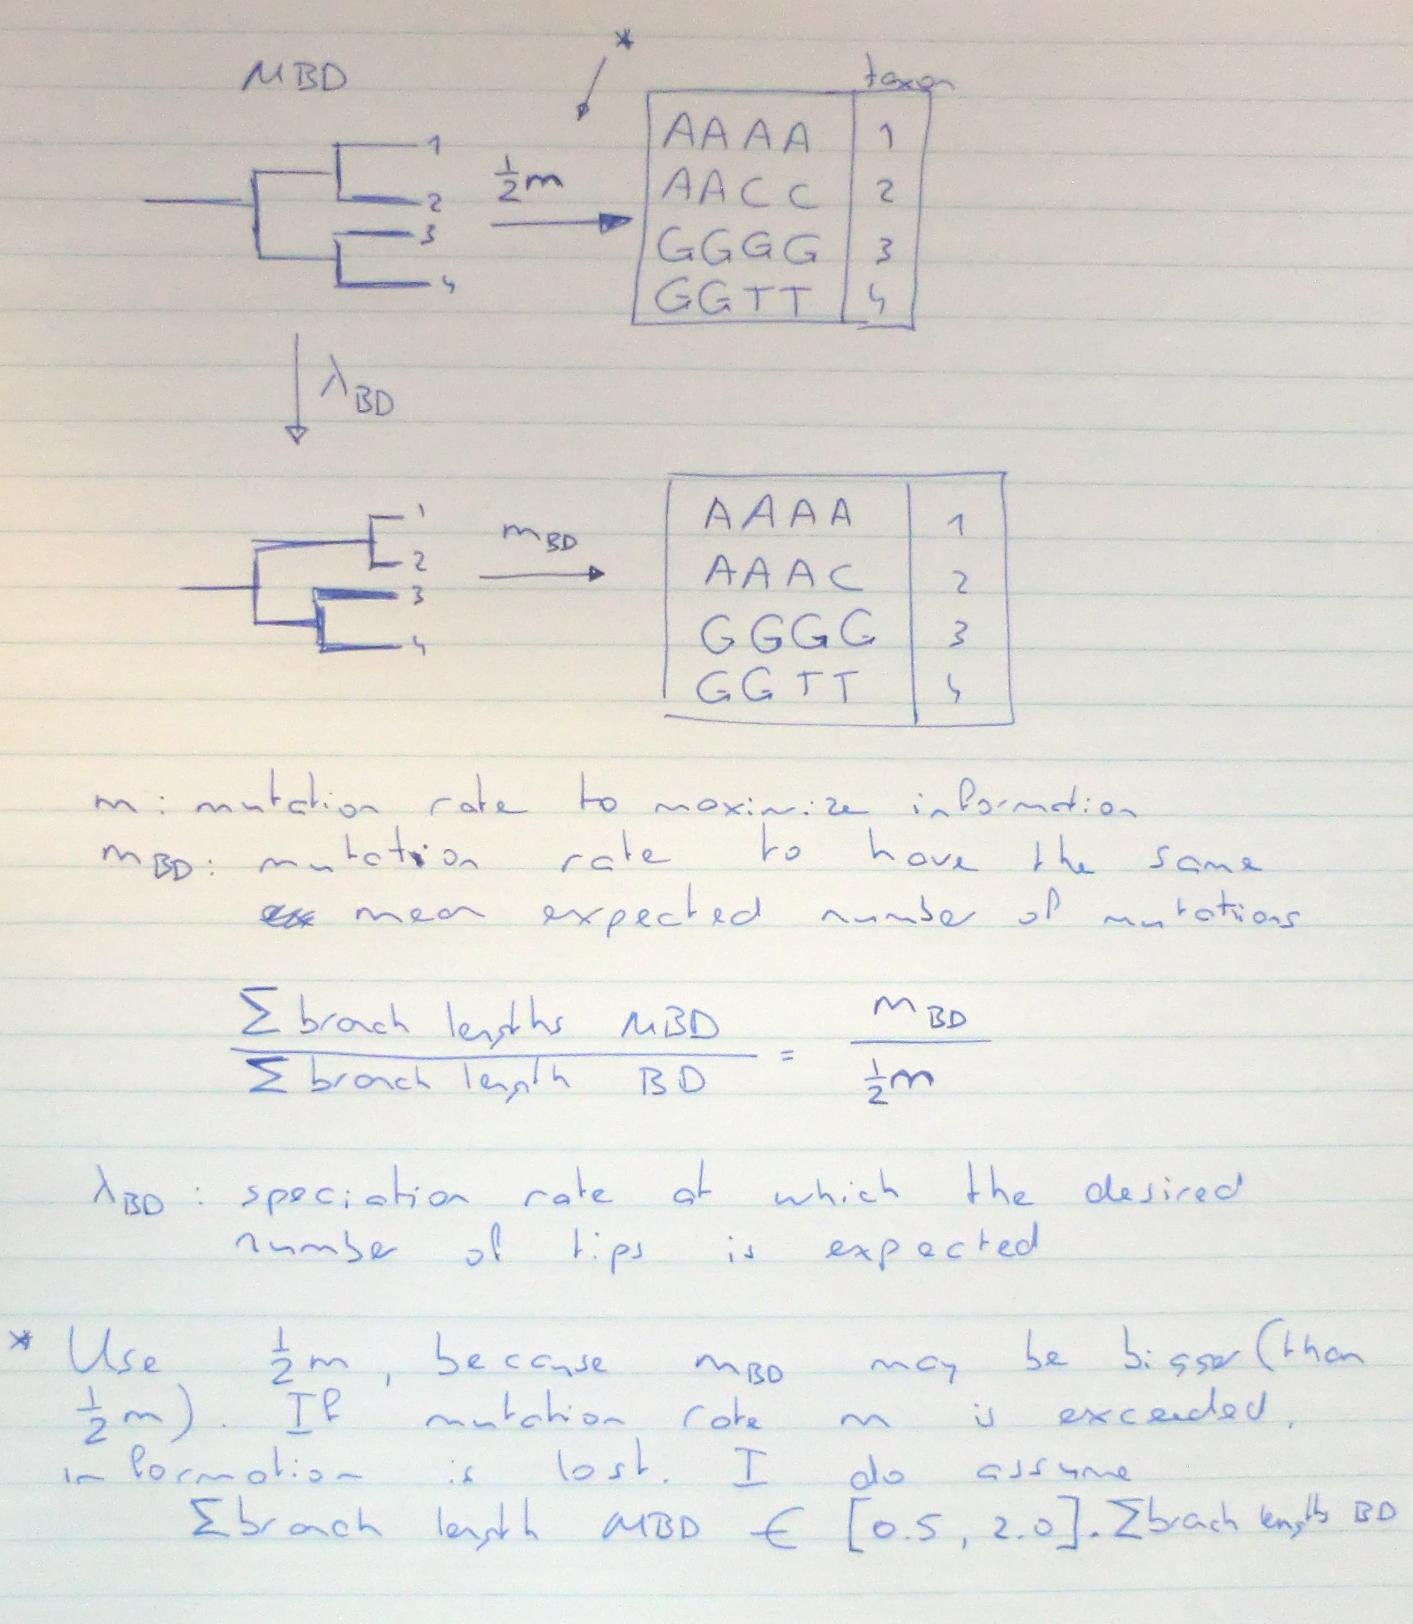
\includegraphics[width=\textwidth]{razzo-figures/fig_mbd.jpg}
  \caption{
    How to create twin trees and alignments. 
    From a focal MBD tree, a twin tree is produced as 
    such: (1) estimate the $\lambda_{BD}$ to get 
    the same expected number of tips, (2) simulate a BD tree 
    with that amount of tips (discard trees with different number of tips), 
    (3) estimate a mutation rate to get an alignment 
    with the same expected number of mutations, (4) simulate alignments 
    with that amount of mutations (discard those that don't, 
    the picture shows an alignment that should be discarded) 
  }
\end{figure}

\item We explained how we set the parameters for each twin BD tree. 
Using this rules we generate a BD dataset. 
We repeat the analysis, producing alignments for each tree 
and subsequently using BEAST to produce a posterior for each of them.

\subsection{Measuring the inference error}

\item So far we have simulated two datasets of trees under the two models: 
$\{T_{i}^{BD}\}_{i=1}^{N_{S}}$ and $\{T_{i}^{MBD}\}_{i=1}^{N_{S}}$.
We used them to generate a dataset of alignments for each model: $\{X^{BD}_{i}\}_{i=1}^{N_{S}}$ and $\{X^{MBD}_{i}\}_{i=1}^{N_{S}}$. From each dataset we produced a posterior distribution from a BD prior: 
$P_{i}(\theta | X^{BD}_{i}, BD)$ and $P_{i}(\theta | X^{MBD}_{i}, BD)$.
\gio{
  1) We might want to rename the models, e.g. BD = (0) and MBD = (1). 
  These names with capital letters are too big and ugly;
}
\richel{
  I would strongly prefer MBD and BD, as I feel replacing the big ugly 
  capital letters by short pretty numbers hurts readability even more 
}

\item To compare the results for the two models we measure the inference 
error using the nLTT statistic between known/true tree and 
posterior/inferred trees (\cite{nltt}). 
To obtain such statistics the procedure is the following:

- From each tree $T_{i,j}^{M}$ (with $j=1,...,N_{S}$) 
  belonging to the posterior $P_{i}(\theta | X^{M}_{i}, BD)$ 
  and relative to the model $M$, we extrapolate the lineage-through-time (LTT), 
  in other words we measure the number of species as a function of 
  time $n_{i,j}(t)$. To allow a comparison we normalize dividing by the 
  maximum number of species of each tree, i.e. the number of tips at the 
  present $N_{i,j}(t)=\frac{n_{i,j}(t)}{n^{max}_{i,j}}$. We then define the 
  nLTT measure as

$nLTT_{i,j} = \int_{0}^{T} | N_{i,j}(t) - N_{T_{i}} | dt$

\gio{I am running out of letters :(}
\richel{Haha! I suggest to use the same equation and symbols 
  as equation 1 in
  the nLTT article of Janzen, Hoehna and Etienne, 2015:
}

$$
\Delta nLTT = \int_{0}^{1} | nLTT_1(t) - nLTT_2{t} | dt
$$

\subsection{Model selection}

We simulate alignments using the simplest nucleotide substitution model (JC69),
the simplest clock model (strict). It is thus imminent to assume these
models in our Bayesian inference. Nevertheless, the phylogeny the alignment
was based on, could have followed either an MBD or BD tree model, 
where we in both cases assume a BD tree model. This will have 
an unknown effect on our inference: it may theoretically be that an MBD model
generates (a tree that generates) an alignment in which a different site 
and/or clock model is favored. 

We investigate this by measuring if the generative model (with the simplest
nucleotide substitution and simplest clock model) is indeed selected 
to be the best fitting model. 
To be precise, we look at the model 
with the highest marginal likelihood 
(also called evidence \cite{mackay2003information}),
$f(D|M)$, which is the probability of the data D given model M.
In the context of this research, D consists of the DNA alignment,
and M is the combination of site, clock and tree models.

To estimate the marginal likelihood, 
we use an algorithm named nested sampling \cite{skilling2006nested}.
Nested sampling is attractive to use
in a phylogentic context, as it gives a good estimation,
requires little tuning \cite{maturana2018}.
Nested sampling is available as a BEAST2 package
and can be used by babette \cite{babette}.

The nested sampling algorithm stops its run 
when the marginal likelihood estimation error 
reaches below a certain tolerance.  
Similar to \cite{maturana2018},
we use a (relative) error tolerance $\epsilon$ of $10^{-13}$,
1 particle to explore the parameter space
and 100 active points. 
To achieve the latter, we use the MCMC chain length $L_c$ of 1M 
(as also used in the parameter estimates),
and a sub-chain length $L_{sc}$ of 10K.

The models we use in our model comparison are the four combinations
of two site models and two clock models. We use the JC69 site model, which
is the (generative and) simplest model and GTR, the site model with most
degrees of freedom. For the clock models, we use the strict clock model,
which is the (generative and) simplest clock model, and the RLN clock model.
\richel{Could also just be all site models and clock models = 8 models}

From these four marginal likelihood estimates, we calculate the weight of
the generative model and plot this in figure 2. We do this for both the 
alignments derived from the MBD tree and the BD twin tree. We expect that
the generative model has the heighest weight in both the MBD and BD alignments.
We expect this weight to be higher in the BD alignments.

\end{itemize}